\documentclass{article}

\usepackage{ctex}
\usepackage[top=0.7in,bottom=0.7in,left=0.5in,right=0.5in]{geometry}
\usepackage{array}
\usepackage{multirow}
\usepackage{graphicx}
\usepackage{fancyhdr}
\usepackage{lastpage}
\usepackage{extramarks}
\usepackage{amsmath}
\usepackage{listings}
\usepackage{fontspec}
\newfontfamily\consolas{Consolas}
\usepackage{xcolor} % 定制颜色
\definecolor{mygreen}{rgb}{0,0.6,0}
\definecolor{mygray}{rgb}{0.5,0.5,0.5}
\definecolor{mymauve}{rgb}{0.58,0,0.82}
\lstset{ %
backgroundcolor=\color{white},      % choose the background color
basicstyle=\footnotesize\ttfamily,  % size of fonts used for the code
columns=fullflexible,
tabsize=4,
breaklines=true,               % automatic line breaking only at whitespace
captionpos=b,                  % sets the caption-position to bottom
commentstyle=\color{mygreen},  % comment style
escapeinside={\%*}{*)},        % if you want to add LaTeX within your code
keywordstyle=\color{blue},     % keyword style
stringstyle=\color{mymauve}\ttfamily,  % string literal style
frame=single,
rulesepcolor=\color{red!20!green!20!blue!20},
% identifierstyle=\color{red},
language=c++,
}

\newcommand{\hmwkTitle}{判别回文字符串\ 实验报告}
\newcommand{\hmwkClass}{数据结构}
\newcommand{\hmwkClassInstructor}{}
\newcommand{\hmwkAuthorName}{毛子恒\ 李臻\ 张梓靖}

\pagestyle{fancy}
\lhead{\hmwkAuthorName}
\chead{\hmwkClass\ : \hmwkTitle}
\rhead{\firstxmark}
\lfoot{\lastxmark}
\cfoot{\thepage}
\renewcommand\headrulewidth{0.4pt}
\renewcommand\footrulewidth{0.4pt}

\title{\hmwkClass\ :\hmwkTitle}
\author{\hmwkAuthorName}

\setcounter{tocdepth}{1}

\begin{document}

\maketitle  

\section*{小组成员}

\setlength{\tabcolsep}{9mm}
{
    \begin{table}[htbp]
        \centering
        \begin{tabular}{llll}
            班级:2019211309 & 姓名:毛子恒 & 学号:2019211397 & 分工:代码\ 文档 \\
            
            班级:2019211310 & 姓名:李臻   & 学号:2019211458 & 分工:测试\ 文档 \\
            
            班级:2019211308 & 姓名:张梓靖 & 学号:2019211379 & 分工:文档       \\
        \end{tabular}
    \end{table}
}

\tableofcontents
\newpage

\section{需求分析}

\subsection{题目描述}

回文串:正序表示和逆序表示相同的字符串。

输入一个字符串,判断其是否是回文串。

\subsection{输入描述}

程序从标准输入中读入数据。输入一行一个字符串,以“\#”结束。

输入满足字符串串的长度$LEN\leq 10^6$

\subsection{输出描述}

程序向标准输出中输出结果。

输出分为两种情况:

\begin{enumerate}
    \item 输入合法,程序正常运行结束。此时输出一行一个字符串“YES”或“NO”(不带引号),分别表示该字符串是/不是回文串。
    \item 程序发生运行时错误,比如内存分配失败。此时程序没有输出。
\end{enumerate}

\subsection{样例输入输出}

\subsubsection{样例输入输出1}

【输入】

\begin{lstlisting}[
    basicstyle=\small\consolas]
11121#
\end{lstlisting}

【输出】

\begin{lstlisting}[
    basicstyle=\small\consolas]
NO
\end{lstlisting}

\subsubsection{样例输入输出2}

【输入】

\begin{lstlisting}[
    basicstyle=\small\consolas]
121#
\end{lstlisting}

【输出】

\begin{lstlisting}[
    basicstyle=\small\consolas]
YES
\end{lstlisting}

\subsubsection{样例输入输出3}

【输入】

\begin{lstlisting}[
    basicstyle=\small\consolas]
kndwtgsynmvlrcqctfdcwwscfrdjdrvtyojjoytvrdjdrfcswwcdftcqcrlvmnysgtwdnk#
\end{lstlisting}

【输出】

\begin{lstlisting}[
    basicstyle=\small\consolas]
YES
\end{lstlisting}

\subsubsection{样例输入输出4}

【输入】

\begin{lstlisting}[
    basicstyle=\small\consolas]
adllaspkbqoytsfxpxwnxvljdmzyyfnlbjnomgxcnsnadllaspkbqoytsfxpxwnxvljdmzyyfnlbjnomgxcnsn#
\end{lstlisting}

【输出】

\begin{lstlisting}[
    basicstyle=\small\consolas]
NO
\end{lstlisting}

\subsection{程序功能}

程序判别输入的字符串是否是回文串。

\section{概要设计}

\subsection{问题解决的思路}

根据栈先进后出和队列先进先出的性质,输入时将元素同时入队、入栈,之后同时出队、出栈,由于出队顺序是正序,出栈顺序是逆序,只需要比较每次出队和出栈元素是否相同即可判断字符串是否是回文串。

此题中栈实现了初始化、判空、入栈、出栈、释放空间这五种操作;队列分别采用顺序和链式两种方式实现了初始化、判空、入队、出队、释放空间这五种操作。

\subsection{栈的定义}

\begin{lstlisting}[language={C},
    numbers=left,
    numberstyle=\tiny\consolas,
    basicstyle=\small\consolas]
//数据对象
typedef char ElemType;

typedef struct stack
{
    ElemType * top;
    ElemType * base;
    int stacksize;
} Stack;

/*
 * 操作:初始化栈,分配空间
 * 后件:s指向一个空栈
 */
void initStack(Stack * s);

/*
 * 操作:判断栈是否为空
 * 前件:s是一个栈
 * 后件:如果该栈为空,返回true;否则返回false
 */
bool isStackEmpty(Stack s);

/*
 * 操作:将数据元素入栈
 * 前件:s指向一个栈
 * 后件:如果入栈成功,item成为栈顶元素;如果入栈之前该栈已满,则重新分配空间
 */
void pushStack(Stack * s, ElemType item);

/*
 * 操作:获取栈顶元素
 * 前件:s是一个栈
 * 后件:如果该栈不为空,返回栈顶元素
 */
ElemType getStackTop(Stack s);

/*
 * 操作:栈顶元素出栈
 * 前件:s指向一个栈
 * 后件:如果该栈不为空,栈顶元素出栈,返回这个出栈的元素
 */
ElemType popStack(Stack * s);

/*
 * 操作:释放栈空间
 * 前件:s指向一个栈
 * 后件:释放该栈的空间
 */
void destroyStack(Stack * s);
\end{lstlisting}

\subsection{队列的定义(顺序)}

\begin{lstlisting}[language={C},
    numbers=left,
    numberstyle=\tiny\consolas,
    basicstyle=\small\consolas]
//数据对象
typedef char ElemType;

typedef struct queue
{
    ElemType * front;
    ElemType * rear;
    ElemType * base;
    int queuesize;
} Queue;

/*
 * 操作:初始化队列,分配空间
 * 后件:q指向一个空队列
 */
void initQueue(Queue * q);

/*
 * 操作:判断队列是否为空
 * 前件:q是一个队列
 * 后件:如果该队列为空,返回true;否则返回false
 */
bool isQueueEmpty(Queue q);

/*
 * 操作:将数据元素入队
 * 前件:q指向一个队列
 * 后件:如果入队成功,item成为队尾元素;如果入队之前该队列已满,则重新分配空间
 */
void pushQueue(Queue * q, ElemType item);

/*
 * 操作:队首元素出队
 * 前件:q指向一个队列
 * 后件:如果该队列不为空,队首元素出栈,返回这个出队的元素
 */
ElemType popQueue(Queue * q);

/*
 * 操作:释放队列空间
 * 前件:q指向一个队列
 * 后件:释放该队列的空间
 */
void destroyQueue(Queue * q);
\end{lstlisting}

\subsection{队列的定义(链式)}

\begin{lstlisting}[language={C},
    numbers=left,
    numberstyle=\tiny\consolas,
    basicstyle=\small\consolas]
//数据对象
typedef char ElemType;

typedef struct node
{
    ElemType item;
    struct Node * next;
} Node;

typedef struct queue
{
    Node * front, * rear;
} Queue;

/*
 * 操作:初始化队列
 * 后件:q指向一个空队列
 */
void initQueue(Queue * q);

/*
 * 操作:判断队列是否为空
 * 前件:q是一个队列
 * 后件:如果该队列为空,返回true;否则返回false
 */
bool isQueueEmpty(Queue q);

/*
 * 操作:将数据元素入队
 * 前件:q指向一个队列
 * 后件:如果入队成功,item成为队尾元素
 */
void pushQueue(Queue * q, ElemType item);

/*
 * 操作:队首元素出队
 * 前件:q指向一个队列
 * 后件:如果该队列不为空,队首元素出队,并且释放其占用的空间,返回这个出队的元素
 */
ElemType popQueue(Queue * q);

/*
 * 操作:释放队列空间
 * 前件:q指向一个队列
 * 后件:释放该队列的空间
 */
void destroyQueue(Queue * q);
\end{lstlisting}

\subsection{主程序的流程}

\begin{enumerate}
    \item 初始化栈和队列
    \item 输入,元素入栈和队列
    \item 每次从栈顶和队首取出元素,并且比较是否相同,重复执行直到队列或栈为空
    \item 输出
    \item 释放空间
\end{enumerate}

\subsection{各程序模块之间的层次关系}

程序模块层次关系图如图1图二。

\begin{figure}[htbp]
    
    \centering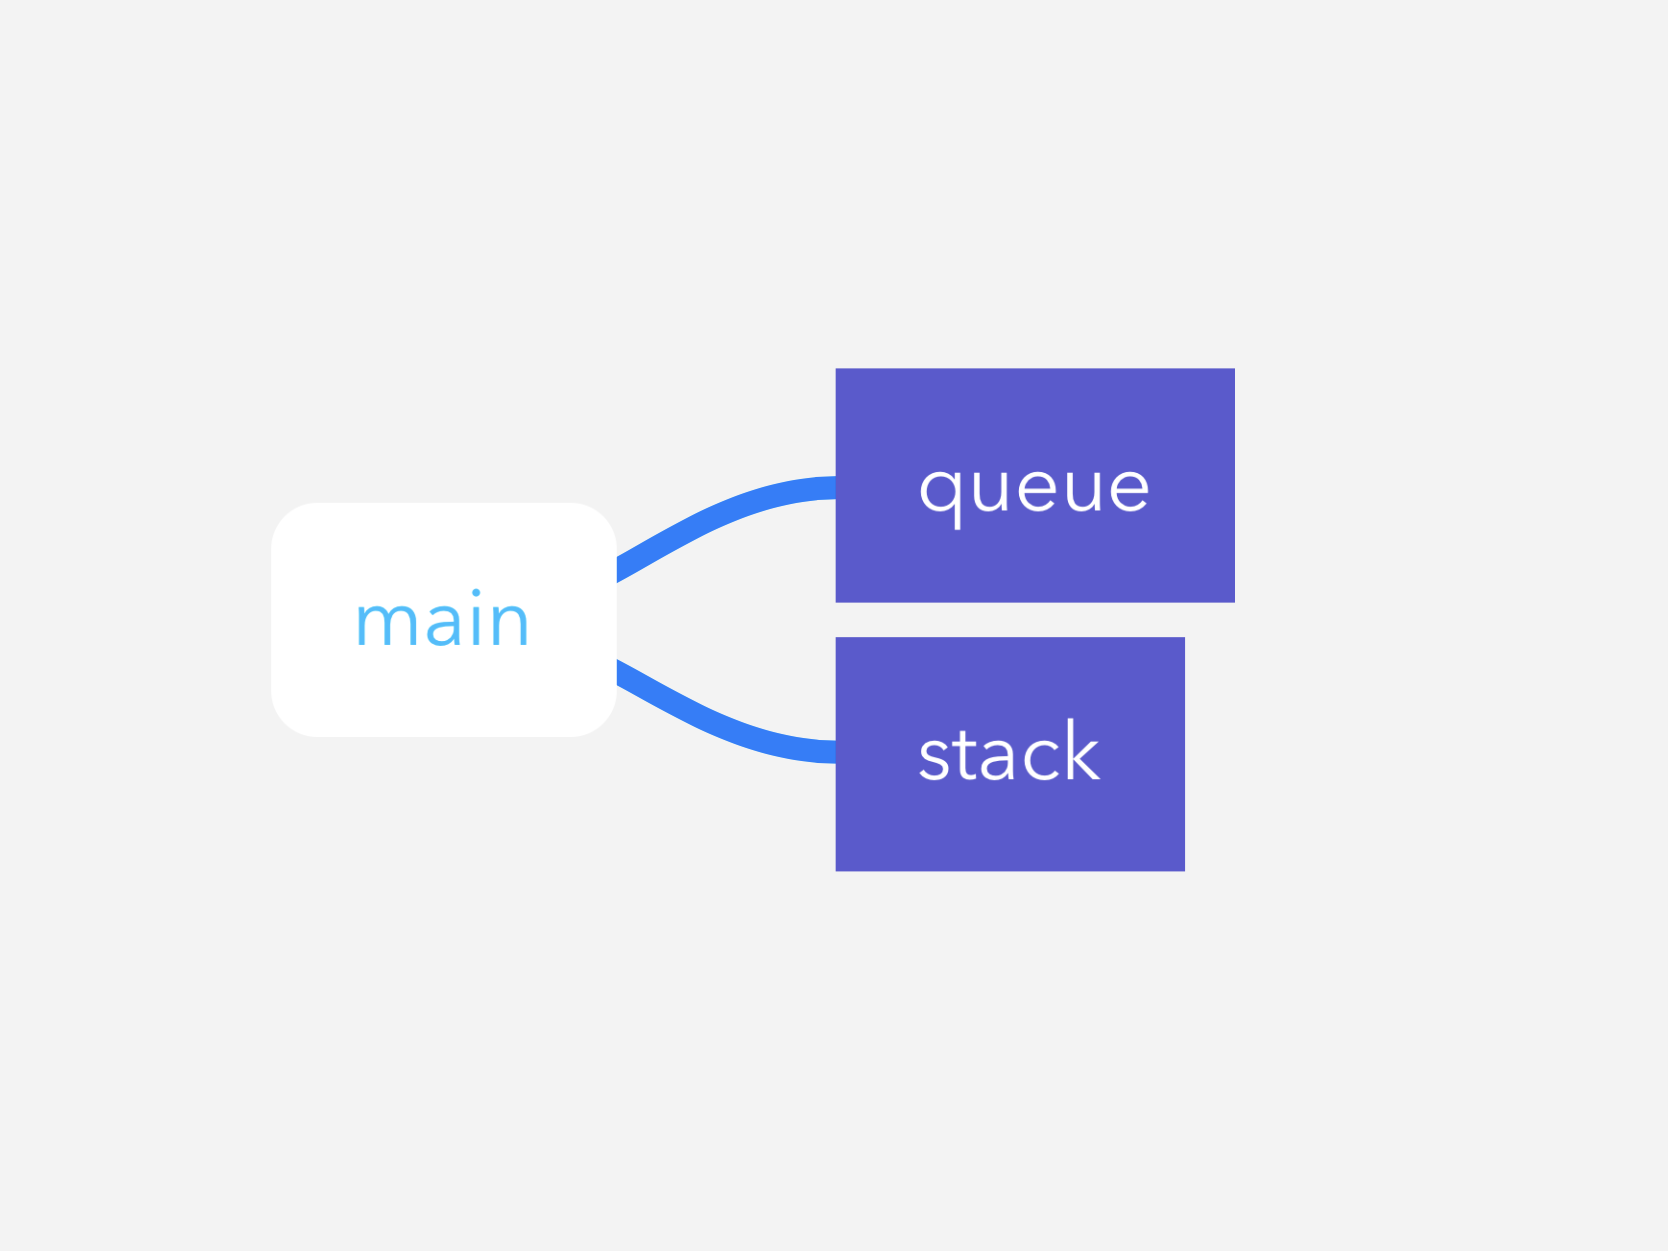
\includegraphics[width=0.4\textwidth]{./Images/pic2_2_1.png}
    
    \caption{程序模块层次关系}
    
\end{figure}

\begin{figure}[htbp]
    
    \centering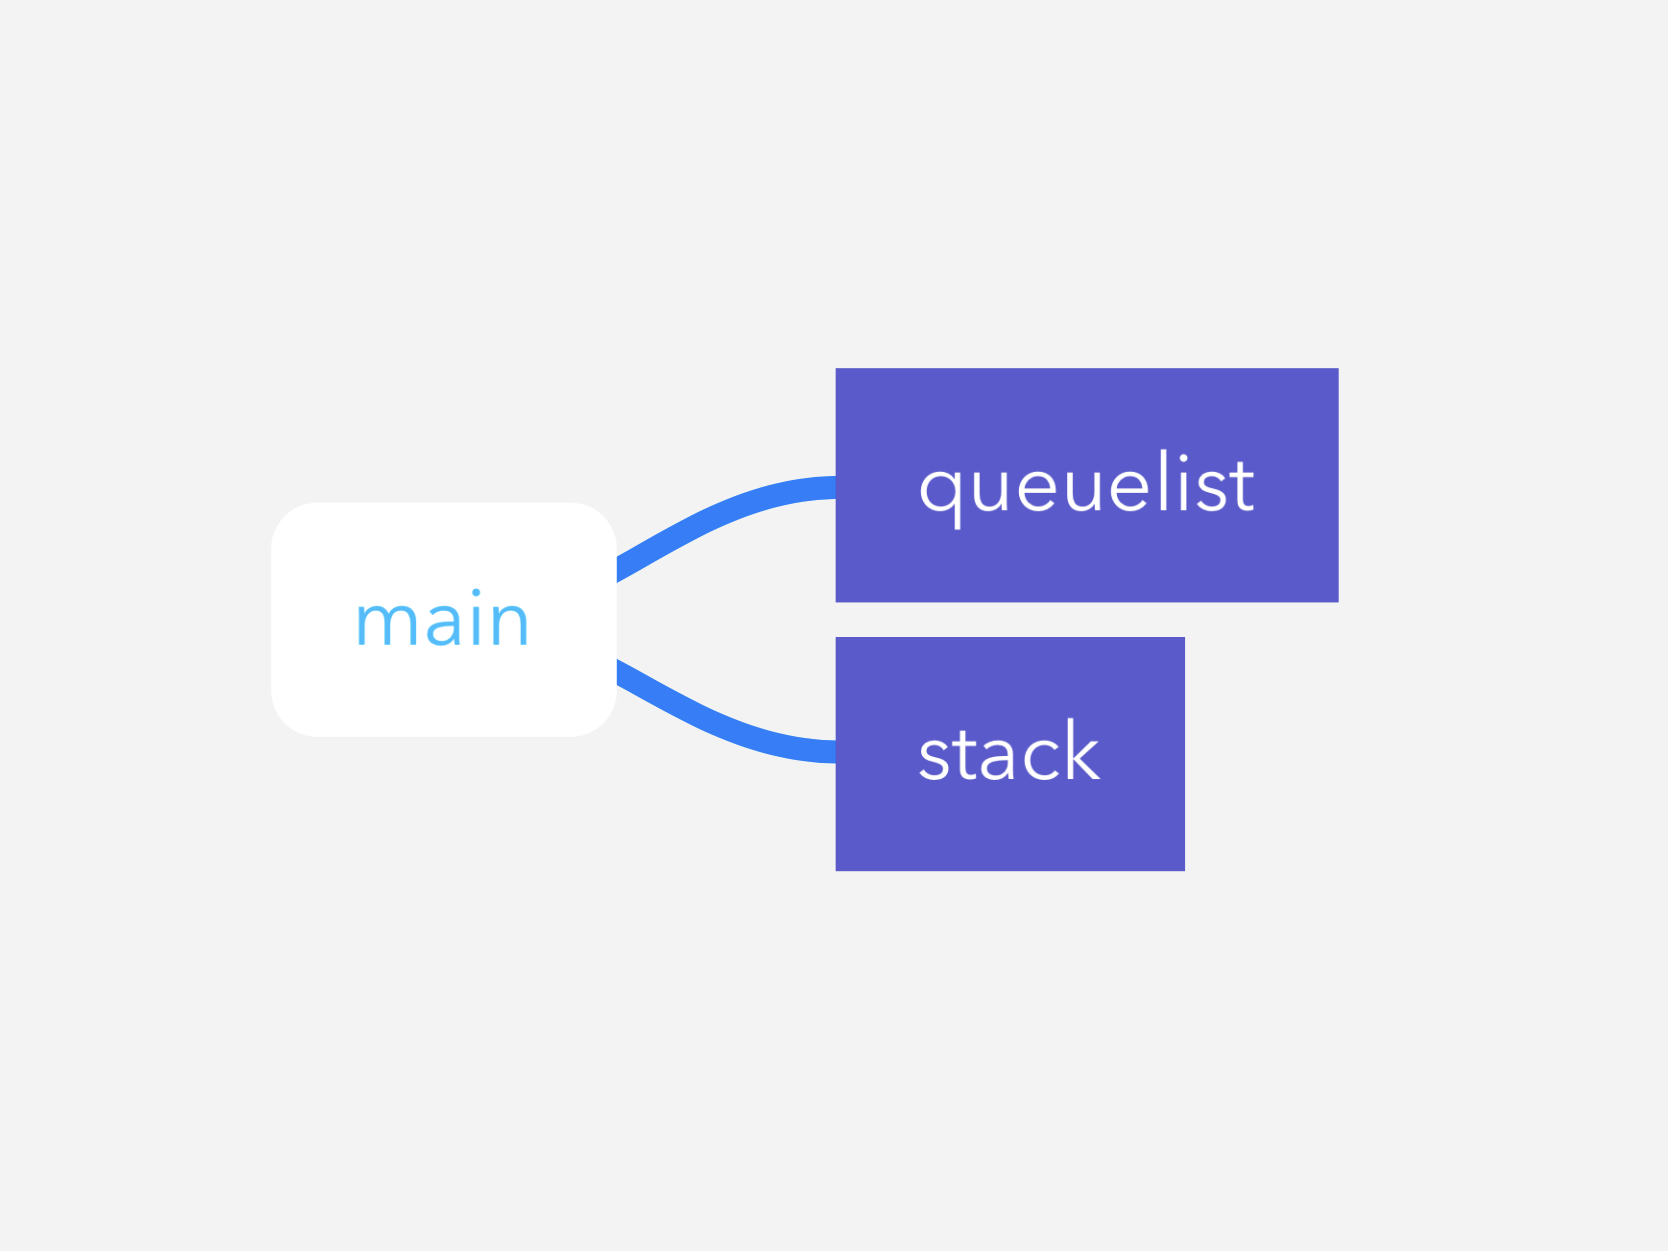
\includegraphics[width=0.4\textwidth]{./Images/pic2_2_2.png}
    
    \caption{程序模块层次关系}
    
\end{figure}

\section{详细设计}

\subsection{栈的实现}

栈设计中基本操作的伪代码算法如下:
\begin{lstlisting}[language={C},
    numbers=left,
    numberstyle=\tiny\consolas,
    basicstyle=\small\consolas]
void Stack(Stack * s) // 初始化栈
{    
    给*s分配内存
    if (*s内存分配失败) // 空间分配失败
        异常退出
    s->top <- s->base
    s->stacksize <- STACKINCREASESIZE // 初始栈空间为STACKINCREASESIZE
}

bool isStackEmpty(Stack s)// 判断栈是否为空
{
    if (s栈为空) 返回1
    else 返回0
}

void pushStack(Stack * s, ElemType item)// 将数据元素入栈
{
    if (s栈满) 
    {
        分配给s更多的空间
        if (s空间分配失败)
            异常退出
        s->top <- s->base + s->stacksize
        s->stacksize <- s->stacksize + STACKINCREASESIZE
    }
    item入栈
}

ElemType popStack(Stack * s)// 栈顶元素出栈
{
    if (栈为空)
        返回异常 
    返回 *(--s->top) // 返回栈顶元素,并且top减1
}

void destroyStack(Stack * s)// 释放栈空间
{
    释放s->base
    s->base <- NULL
    s->top <- NULL
    s->stacksize <- 0
}
\end{lstlisting}

\subsection{队列的实现(顺序)}

\begin{lstlisting}[language={C},
    numbers=left,
    numberstyle=\tiny\consolas,
    basicstyle=\small\consolas]
    
void initQueue(Queue * q) // 初始化队列,分配空间
{
    给q->base分配内存
    if (q->base 内存分配失败) // 空间分配失败
        异常退出
    q->front = q->rear <- q->base //q指向一个空队列
    q->queuesize <- QUEUEINCREASESIZE
}

bool isQueueEmpty(Queue q) // 判断队列是否为空
{
    if (q.front 和 q.rear 相等) 返回1
    else 返回0
}

void pushQueue(Queue * q, ElemType item) // 将数据元素入队
{
    if (q->rear 减 q->base 的差与 q->queuesize相等) // 队列满
    {
        定义整型temp1 <- q->front - q->base
        分配给q->base更多的内存
        if (内存分配失败)
            异常退出 
        q->front <- q->base + temp1
        q->rear <- q->base + q->queuesize
        q->queuesize <- q->queuesize + QUEUEINCREASESIZE
    }
    item入队
}

ElemType popQueue(Queue * q) // 队首元素出队
{
    if (*q队列为空)
        异常退出
    返回 *(q->front++)
}

void destroyQueue(Queue * q)// 释放队列空间
{
    释放q->base
    q->base = q->front = q->rear <- NULL
    q->queuesize <- 0
}
\end{lstlisting}

\subsection{队列的实现(链式)}

\begin{lstlisting}[language={C},
    numbers=left,
    numberstyle=\tiny\consolas,
    basicstyle=\small\consolas]
    
void initQueue(Queue * q)// 初始化队列
{
    定义* newNode并为其分配内存
    if (newNode内存分配失败)
        异常退出
    q->front = q->rear <- newNode;
    newNode->item <- 0; // 创建空的头结点
    newNode->next <- NULL;
}

bool isQueueEmpty(Queue q) // 判断队列是否为空
{
    if (q.front 和 q.rear 相等) 返回1
    else 返回0
}

void pushQueue(Queue * q, ElemType item) // 将数据元素入队
{
    定义* newNode并为其分配内存
    if (newNode内存分配失败)
        异常退出
    newNode->item <- item;
    newNode->next <- NULL; // 将newNode作为链表的尾元素
    q->rear->next <- newNode;
    q->rear <- newNode; // 将队列尾指向newNode
}

ElemType popQueue(Queue * q) // 队首元素出队
{
    定义Node* nextNode 指向 q->front->next
    定义ElemType item <- nextNode->item // 出队的是队首指针的下一个元素
    释放q->front
    q->front <- nextNode
    返回 item
}

void destroyQueue(Queue * q)// 释放队列空间
{
    while (队列不为空) 
        删除队列中剩余的节点
    释放q->front
    q->front = q->rear <- NULL
}
\end{lstlisting}

\subsection{函数的调用关系图}

函数调用关系图如图3。

\begin{figure}[htbp]
    
    \centering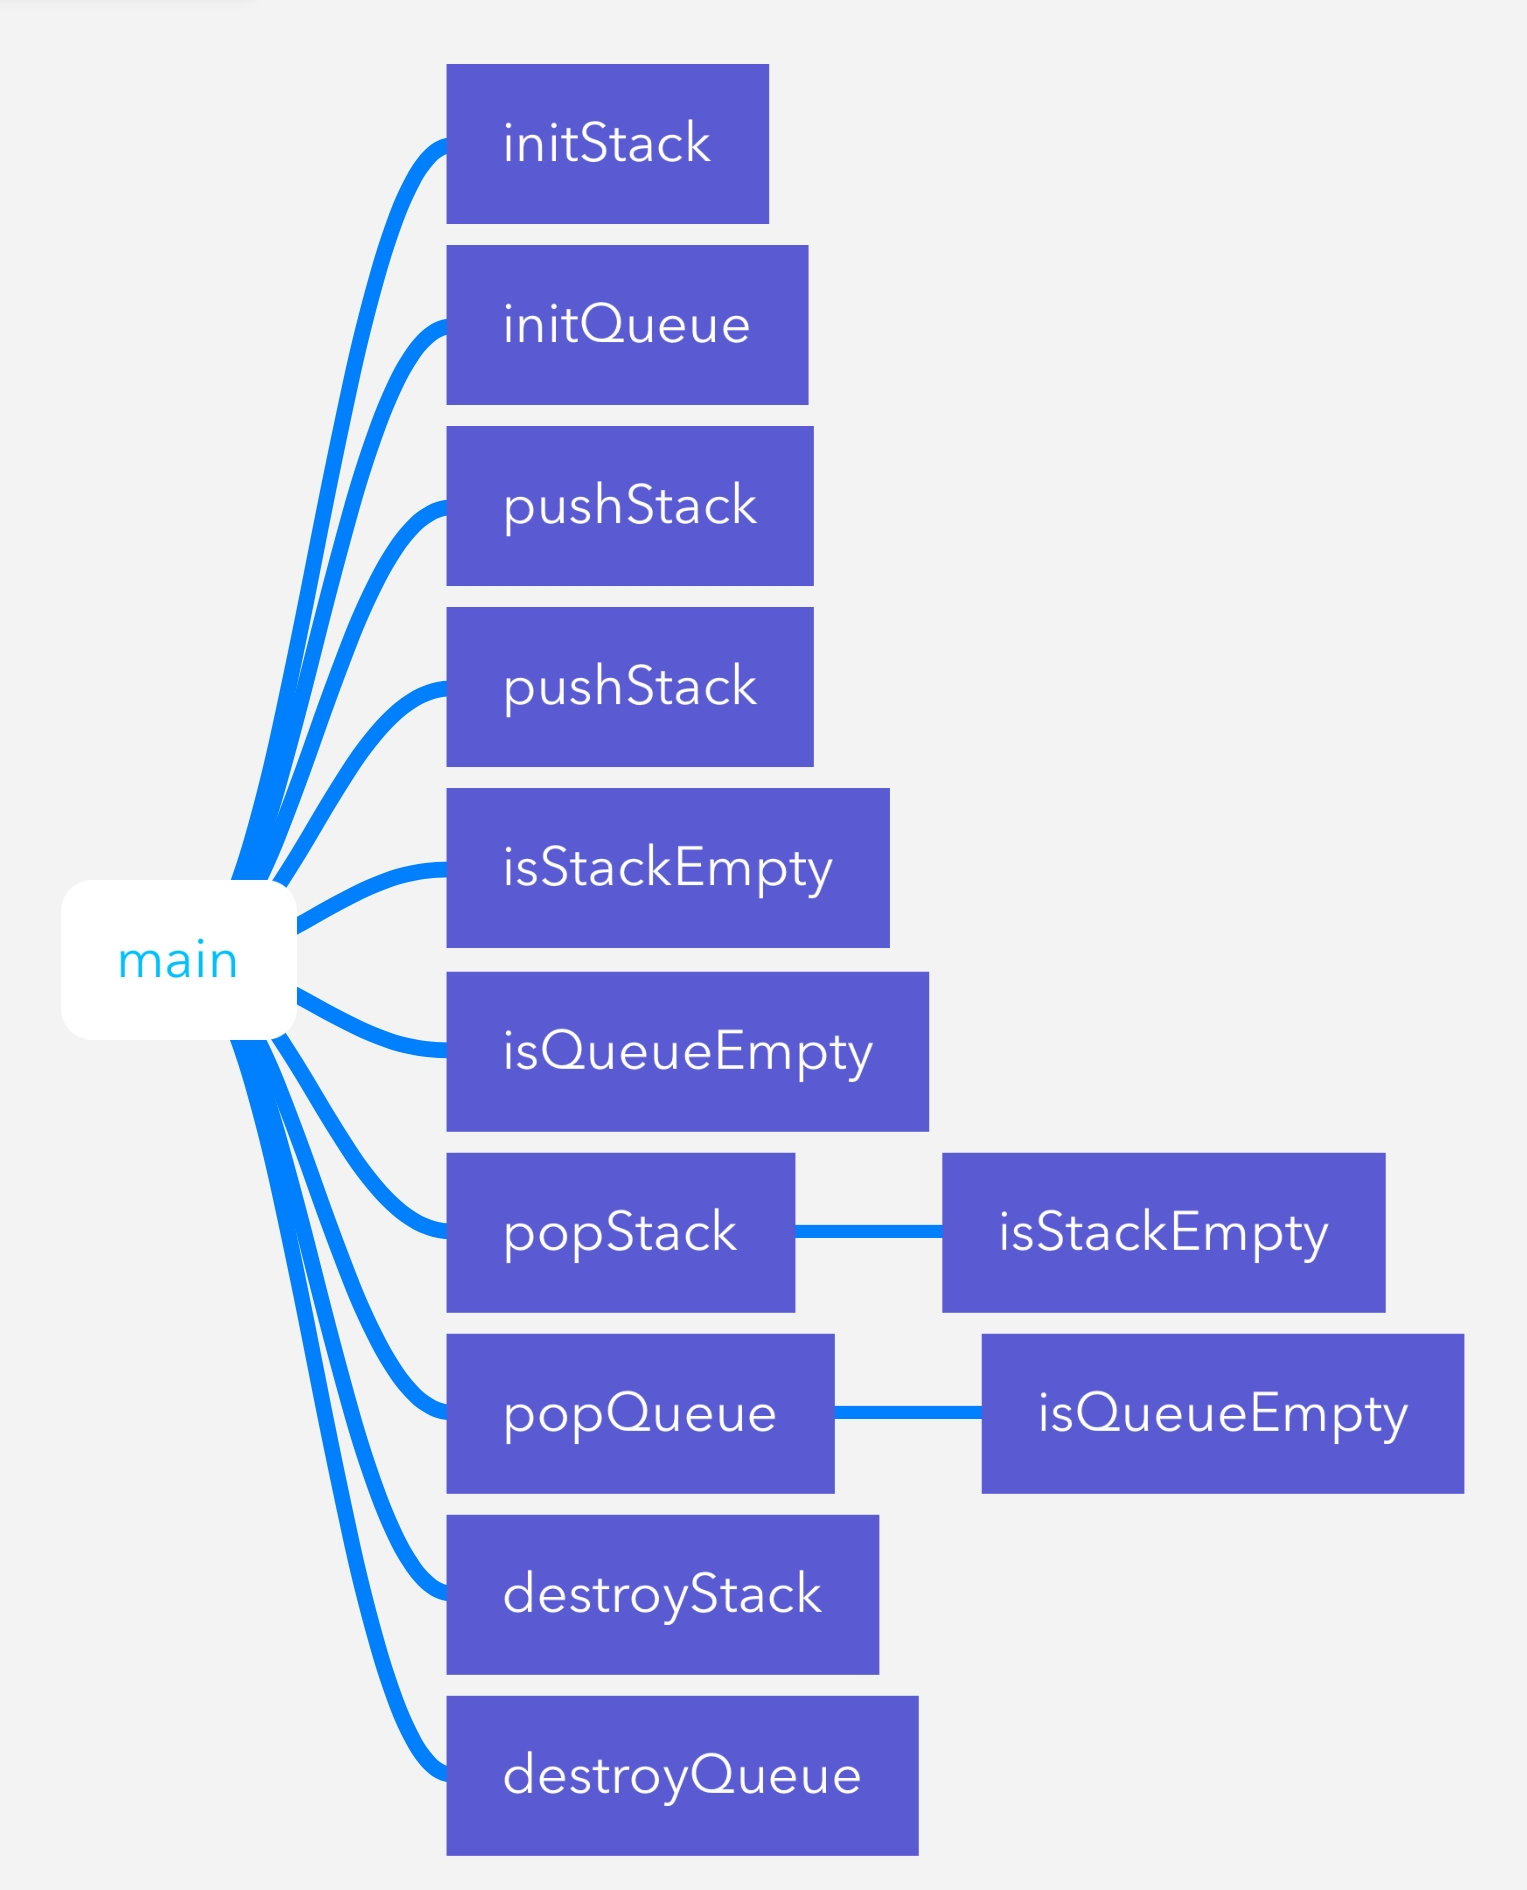
\includegraphics[width=0.4\textwidth]{./Images/pic2_2_3.png}
    
    \caption{函数调用关系图}
    
\end{figure}

\section{调试分析报告}

\subsection{调试过程中遇到的问题和思考}

初步实现后,测试样例时发现对于前导零的情况没有处理,遂增加查询栈顶操作,并且在主程序中增加弹出栈顶0元素的循环。

之后对串全为0的情况增加特判。

对于规模较大的数据测试时发现指针会访问到无效位置,发现是realloc操作之后没有更新$top$指针的位置所致。遂增加更新$top$指针的语句。

\subsection{设计实现的回顾讨论}

队列的链表实现中,$front$指针指向队首元素的前一个位置。

期望输入合法,所以对于输入末尾没有\#的情况没有作处理。

由于不清楚测试用数据的范围大小,$STACKINCREASESIZE$,$QUEUEINCREASESIZE$常量的大小取到100,也就是每次增加100个元素的空间。当输入很大时复杂度可能会比较大。

由于主函数对函数的调用足够严密,所以栈、队列的实现没有考虑不符合前件的情况。

\subsection{算法复杂度分析}

initStack, isStackEmpty, pushStack, getStackTop, popStack, destroyStack函数的时间复杂度均为$O(1)$。

主程序复杂度为$O(n)$,整体时间复杂度为$O(n)$。

\subsection{改进设想的经验和体会}

\subsubsection{改进1}

使用数组实现的回文串判断(testing/test.c):

\begin{lstlisting}[language={C},
    numbers=left,
    numberstyle=\tiny\consolas,
    basicstyle=\small\consolas]
#include <stdio.h>
#include <string.h>

const int MAXN = 1e6 + 10;
int n;
char a[MAXN];

int main()
{
    scanf("%s", a + 1);
    n = strlen(a + 1) - 1;
    for (int i = 1; i <= n / 2; ++i)
        if (a[i] != a[n - i + 1])
        {
            puts("NO");
            return 0;
        }
    puts("YES");
    return 0;
}
\end{lstlisting}

此程序用于测试第三部分。

\section{用户使用说明}

使用gcc编译生成可执行文件。

\begin{lstlisting}[language={bash},
    basicstyle=\small\consolas]
gcc -o main -std=c11 main.c stack.c
\end{lstlisting}

执行可执行文件:

\begin{lstlisting}[language={bash},
    basicstyle=\small\consolas]
./main
\end{lstlisting}

在Windows cmd下:

\begin{lstlisting}[language={bash},
    basicstyle=\small\consolas]
main
\end{lstlisting}

之后通过标准输入输入数据,输入格式参考1.2节的输入描述,结果通过标准输出返回。如果输入合法并且程序正常运行结束,主函数返回值为0。

\section{测试结果}

测试环节分为三个步骤。

\subsection{测试第一部分}

对1.4节给出的样例进行测试。

\subsection{测试第二部分}

测试非法输入和边界条件。

【输入】

\begin{lstlisting}[
    basicstyle=\small\consolas]
1$21#
\end{lstlisting}

【输出】

\begin{lstlisting}[
    basicstyle=\small\consolas]
Please check your input.
\end{lstlisting}

【输入】

\begin{lstlisting}[
    basicstyle=\small\consolas]
0#
\end{lstlisting}

【输出】

\begin{lstlisting}[
    basicstyle=\small\consolas]
0
\end{lstlisting}

【输入】

\begin{lstlisting}[
    basicstyle=\small\consolas]
00000000000000000000#
\end{lstlisting}

【输出】

\begin{lstlisting}[
    basicstyle=\small\consolas]
0
\end{lstlisting}

【输入】

\begin{lstlisting}[
    basicstyle=\small\consolas]
0000000010#
\end{lstlisting}

【输出】

\begin{lstlisting}[
    basicstyle=\small\consolas]
2
\end{lstlisting}

\subsection{测试第三部分}

将原解法与4.4.1节改进解法比对。

测试在macOS\ Catalina\ 10.15.6下进行。

在$LEN<=10$,$LEN<=1000$,$LEN<=1000000$的范围下分别随机生成1000组测试数据,分别传入main和test.py,并且比对两程序的输出。

3000组数据中两程序的输出均相同。

数据生成程序(data.cpp)如下:

\begin{lstlisting}[language={C++},
    numbers=left,
    numberstyle=\tiny\consolas,
    basicstyle=\small\consolas]
#include <bits/stdc++.h>

using namespace std;

const int LEN = 1e6;
char a[LEN + 10];

int main()
{
    srand(time(0));
    int n = rand() % LEN + 1;
    for (int i = 1; i <= n / 2; ++i)
        printf("%c", a[i] = rand() % 26 + 'a');
    if (rand() % 2 == 1)
    {
        for (int i = 1; i <= n / 2; ++i)
            printf("%c", a[i]);
    }
    else
    {
        for (int i = n / 2; i >= 1; --i)
            printf("%c", a[i]);
    }
    puts("#");
    return 0;
}
\end{lstlisting}

比对脚本(chk.sh)如下:

\begin{lstlisting}[language={bash},
    numbers=left,
    numberstyle=\tiny\consolas,
    basicstyle=\small\consolas]
for i in {1..100}
do
    sleep 1
    ./data >in.in
    ./main <in.in >out.out
    ./test <in.in >out1.out
    if ! diff out.out out1.out
    then
        break
    fi
    echo "Correct"
done
\end{lstlisting}

\end{document}
